\documentclass[a4paper,10pt]{article}
\usepackage[utf8]{inputenc}
\usepackage{polski}
\usepackage{graphicx}
\usepackage{listings}
\usepackage[usenames,dvipsnames]{color}
\addtolength{\hoffset}{-1cm}
\addtolength{\voffset}{-2cm}
\addtolength{\textwidth}{2cm}
\addtolength{\textheight}{3cm}
\usepackage{setspace}
\usepackage{indentfirst}
\usepackage{graphicx}
\lstset{
    language=Matlab,
    basicstyle=\scriptsize,
    aboveskip={1.5\baselineskip},
    columns=fixed,
    showstringspaces=false,
    extendedchars=true,
    breaklines=true,
    tabsize=4,
    prebreak = \raisebox{0ex}[0ex][0ex]{\ensuremath{\hookleftarrow}},
    frame=single,
    showtabs=false,
    showspaces=false,
    showstringspaces=false,
    identifierstyle=\ttfamily,
    keywordstyle=\color[rgb]{0,0,1},
    commentstyle=\color[rgb]{0.133,0.545,0.133},
    stringstyle=\color[rgb]{0.627,0.126,0.941},
    numbers=left,
    numberstyle=\tiny,
    stepnumber=1,
    numbersep=5pt,
    captionpos=b,
    escapeinside={\%*}{*)}
}

\def\figurename{Rys.}
\def\lstlistingname{Fun.}

\title{Informatyczne Systemy Sterowania \\ \large Ćwiczenie 5: Sterowanie szybkością transmisji w sieci komputerowej}

\author{Adam Jordanek 168139, Tomasz Klimek 168092}

\begin{document}
\maketitle
\section{Wstęp}\label{sec:wstęp}
\subsection{Cel ćwiczenia}
Celem ćwiczenia jest symulacja systemu zamieszczonego w dokumencie jest to system sterowania ruchem w sieci komputerowej. \\
Cele ćwiczenia: 
\begin{enumerate}
	\item Poznanie problemu sterowania ruchem w sieci komputerowej jako przykładu 
sterowania systemem komputerowym. 
	\item Nabycie umiejętności wykorzystania pakietu Matlab oraz Simulink do symulacji ww. systemu. 
\end{enumerate}
\subsection{Plan badań} 
\begin{enumerate}
	\item Symulacja systemu sterowania szybkością transmisji.
	\item Dobór optymalnego regulatora.
\end{enumerate}
\section{Realizacja planu i wyniki}

%-------------------------------------------------------------------------------------
%                                ZADANIE 1
%-------------------------------------------------------------------------------------
\subsection{Symulacja systemu sterowania szybkością transmisji}

Systemem symulowanym w tym ćwiczeniu będzie system opisany w artykule "\textit{Complete Stability Region
Characterization for PI-AQM}" , czyli system sterujący ruchem w sieci komputerowej. Z powyższego artykułu dla sieci, w której $C$ - przepustowość sieci, $N$ - ilość otwartych sieci TCP, oraz $d$ - opóźnienie pakietów, uzyskaliśmy następującą transmitancję.

\begin{equation} \label{eqn:transO}
	K_{O}(s)={B \over (s + \alpha) (s + \beta)}e^{-sd}
\end{equation}

Gdzie $\alpha = {2N \over d^{2}C}$, $\beta = {1 \over d}$ i $B = {C^2 \over 2N}$.

Regulować system będziemy używając regulatorów z rodziny PID (dzięki uprzejmości prowadzącego zajęcia laboratoryjne tylko P i PID), które opisane są poniższą transmitancją.

\begin{equation} \label{eqn:transR}
	K_{R}(s) = k + {T_{i} \over s} + T_{d}s ,
\end{equation}

Aby zasymulować system w Simulinku musieliśmy wymnożyć mianownik transmitancji obiektu tak, aby można było przedstawić go w postaci 2 bloczków (\textit{Transfer Fnc} i \textit{Transport Delay}).

\begin{equation} \label{eqn:transO}
	K_{O}(s)={B \over s^{2} + (\alpha + \beta)s + \alpha \beta}e^{-sd}
\end{equation}

\newpage
Gotowy schemat służący nam do symulacji przedstawiony jest na poniższym obrazku.

\begin{figure}[!h]
    \centering
	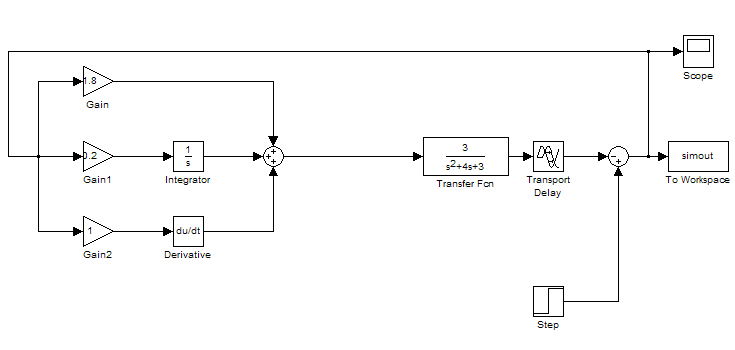
\includegraphics[width=120mm]{CW5-model-systemu.png}
	\caption{Schemat systemu służący nam do symulacji.}
    \label{fig:Rysunek}
\end{figure}

%-------------------------------------------------------------------------------------
%                                ZADANIE 2
%-------------------------------------------------------------------------------------
\subsection{Dobór optymalnego regulatora}

Przy doborze optymalnego regulatora i jego parametrów używaliśmy poniższej prostej funkcji napisanej w Matlabie.

%--------------
%zmieniłem trochę funkcję, żeby była czytelniejsza, z resztą i tak w większości wywoływałem ją dla 3:3,2:2, etc. ;)
%--------------
\begin{lstlisting}[caption=Funkcja testująca system.]
function test(N,C,d,P,I,D)
    load_system('PID.mdl');
    set_param('PID/Gain', 'Gain', num2str(P));   
    set_param('PID/Gain1', 'Gain', num2str(I));   
    set_param('PID/Gain2', 'Gain', num2str(D));
   
    set_param('PID/Transport Delay', 'DelayTime', num2str(d);        
        
    B=C(j+1)/2*N(j+1);
    set_param('PID/Transfer Fcn', 'Numerator', ['[',num2str(B),']']);        
        
    %Alfa i Beta 
    a=2*N/((d^2)*C);
    b=1/d;
    set_param('PID/Transfer Fcn', 'Denominator', ['[1 ',num2str(a+b),' ',num2str(a*b),']']);        
        
    sim('PID.mdl');
    wy = simout.signals.values;    
  	plot(tout, wy, '-k');
end
\end{lstlisting}

Aby zacząć testować system wybraliśmy parametry obiektu, dla których przeprowadzaliśmy dalsze testy, Mianowicie wybraliśmy $N = 3$, $C = 2$, $d = 1$

\newpage
\subsubsection{Regulator P}

Symulując system z regulatorem P wywoływaliśmy funkcję test, podając wartość $0$ dla parametrów $I$, oraz $D$. W ten sposób uzyskalismy poniższe wykresy.

\begin{figure}[!h]
    \centering
	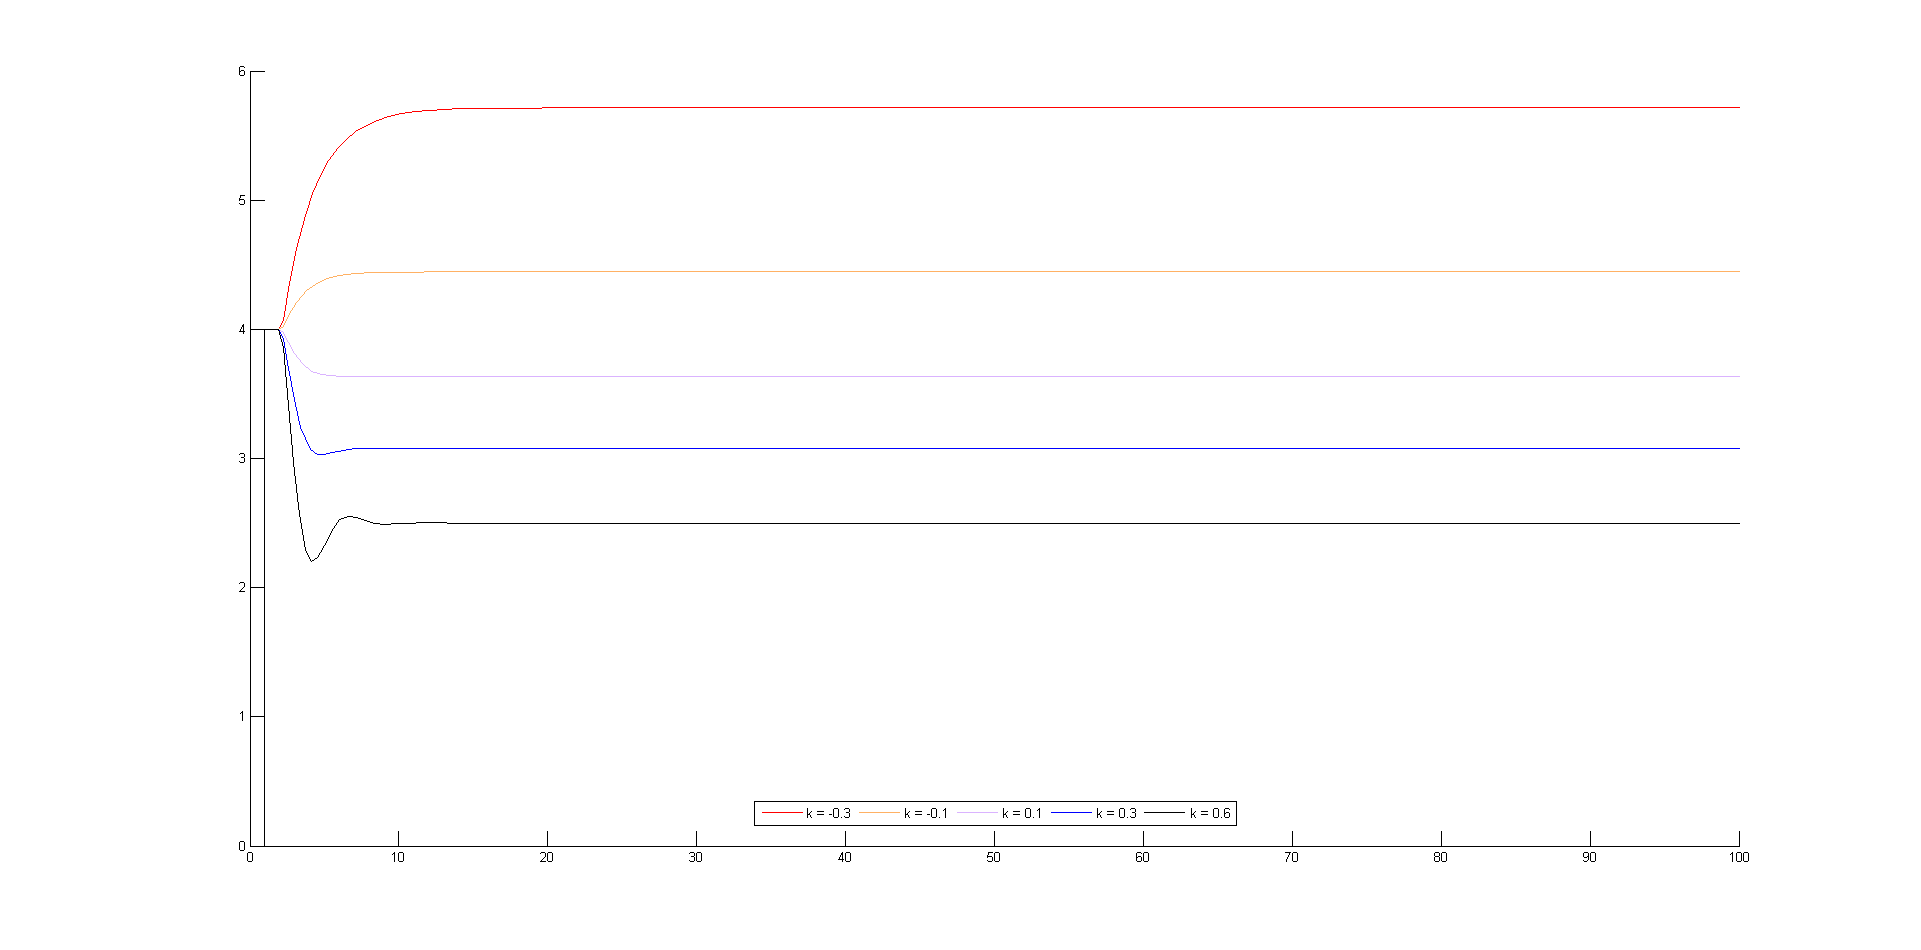
\includegraphics[width=120mm]{CW5-N3C2d1-k-03-06.png}
	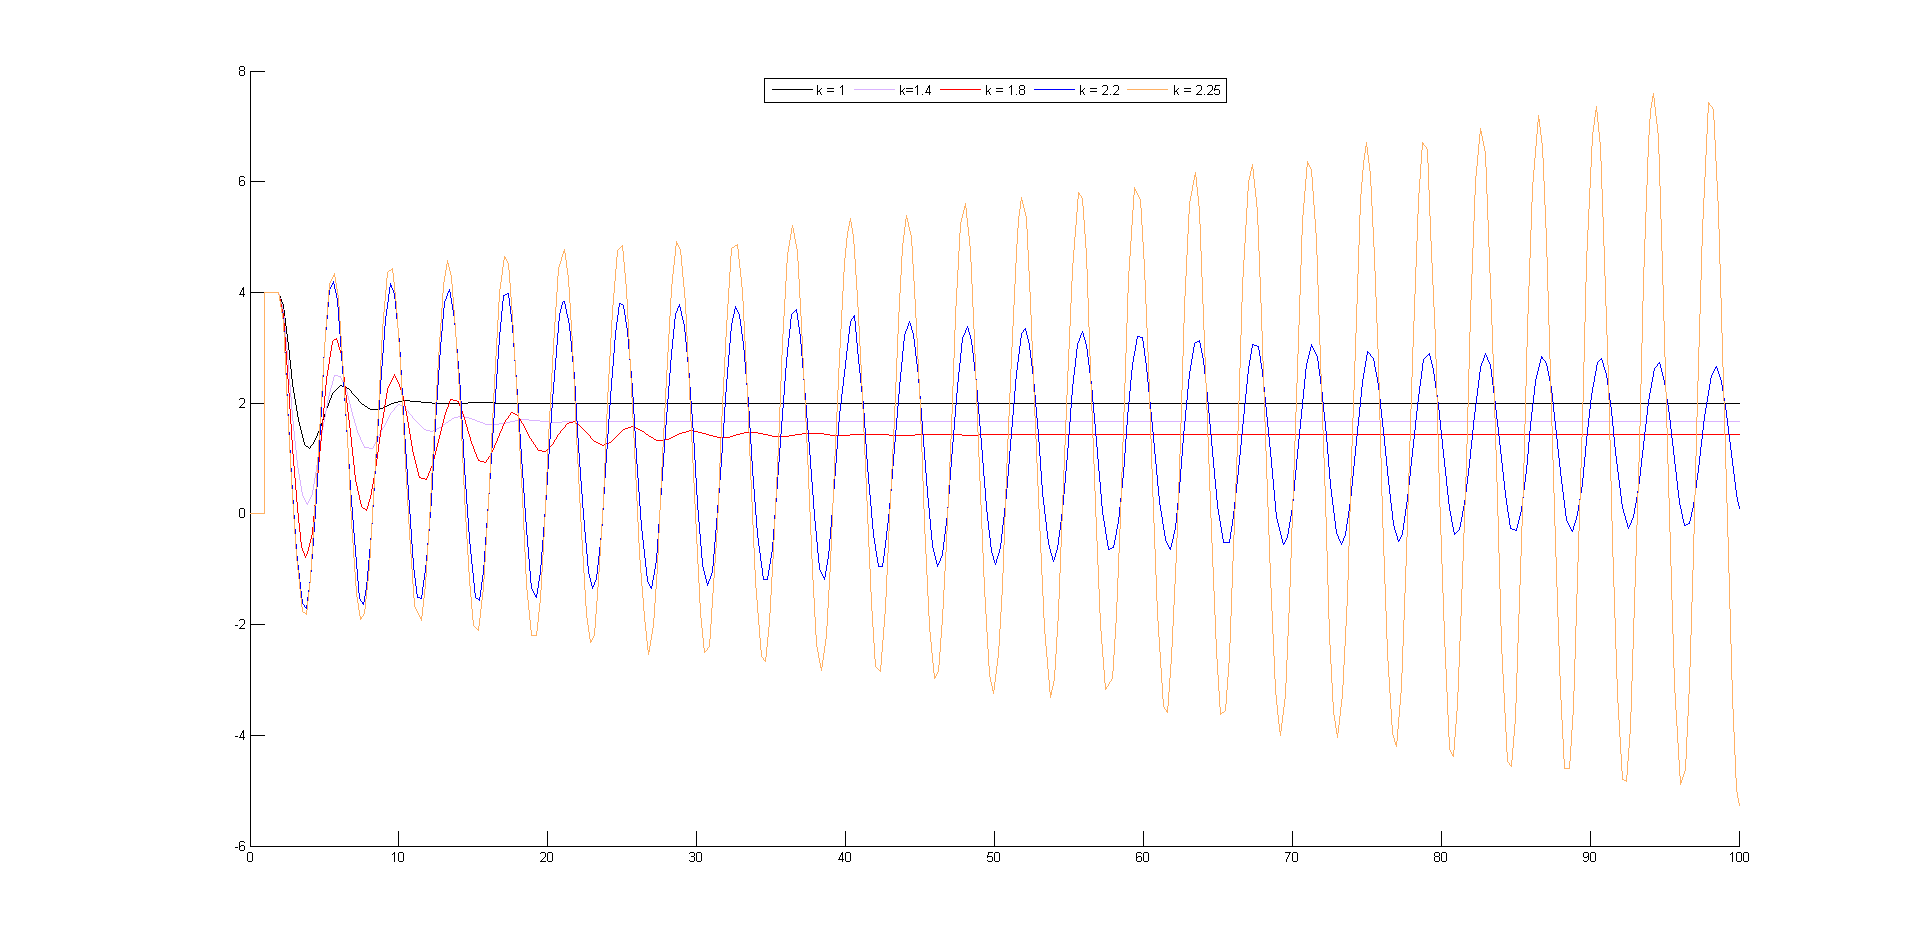
\includegraphics[width=120mm]{CW5-N3C2d1-k1-225.png}
	\caption{Wykresy przebiegu błędu regulacji przy zmianie parametru $k$}
    \label{fig:symulacjaP}
\end{figure}

Na wykresach \ref{fig:symulacjaP} możemy zaobserwować, że:
\begin{itemize}
	\item Dla ujemnych wartości parametru $k$ wartość błędu szybko stabilizuje się na pewnym poziomie. Poziom ten jest tym większy, im mniejsza jest wartość parametru $k$.
	\item Dla małych ($<1.8$) dodatnich wartości parametru $k$ wartość błędu również szybko stabilizuje się na pewnym poziomie, a poziom ten jest tym mniejszy, im większa jest wartość parametru $k$.
	\item Dla większych wartości dodatnich ($>1.8$) wykres wartości błędu regulacji wolniej stabilizuje się, a dla $k \approx 2.23$ przybiera kształt drgań o stałej amplitudzie. Powyżej tej wartości amplituda drgań z czasem rośnie.
\end{itemize}
\newpage
\subsubsection{Regulator PID}
\begin{figure}[!h]
    \centering
	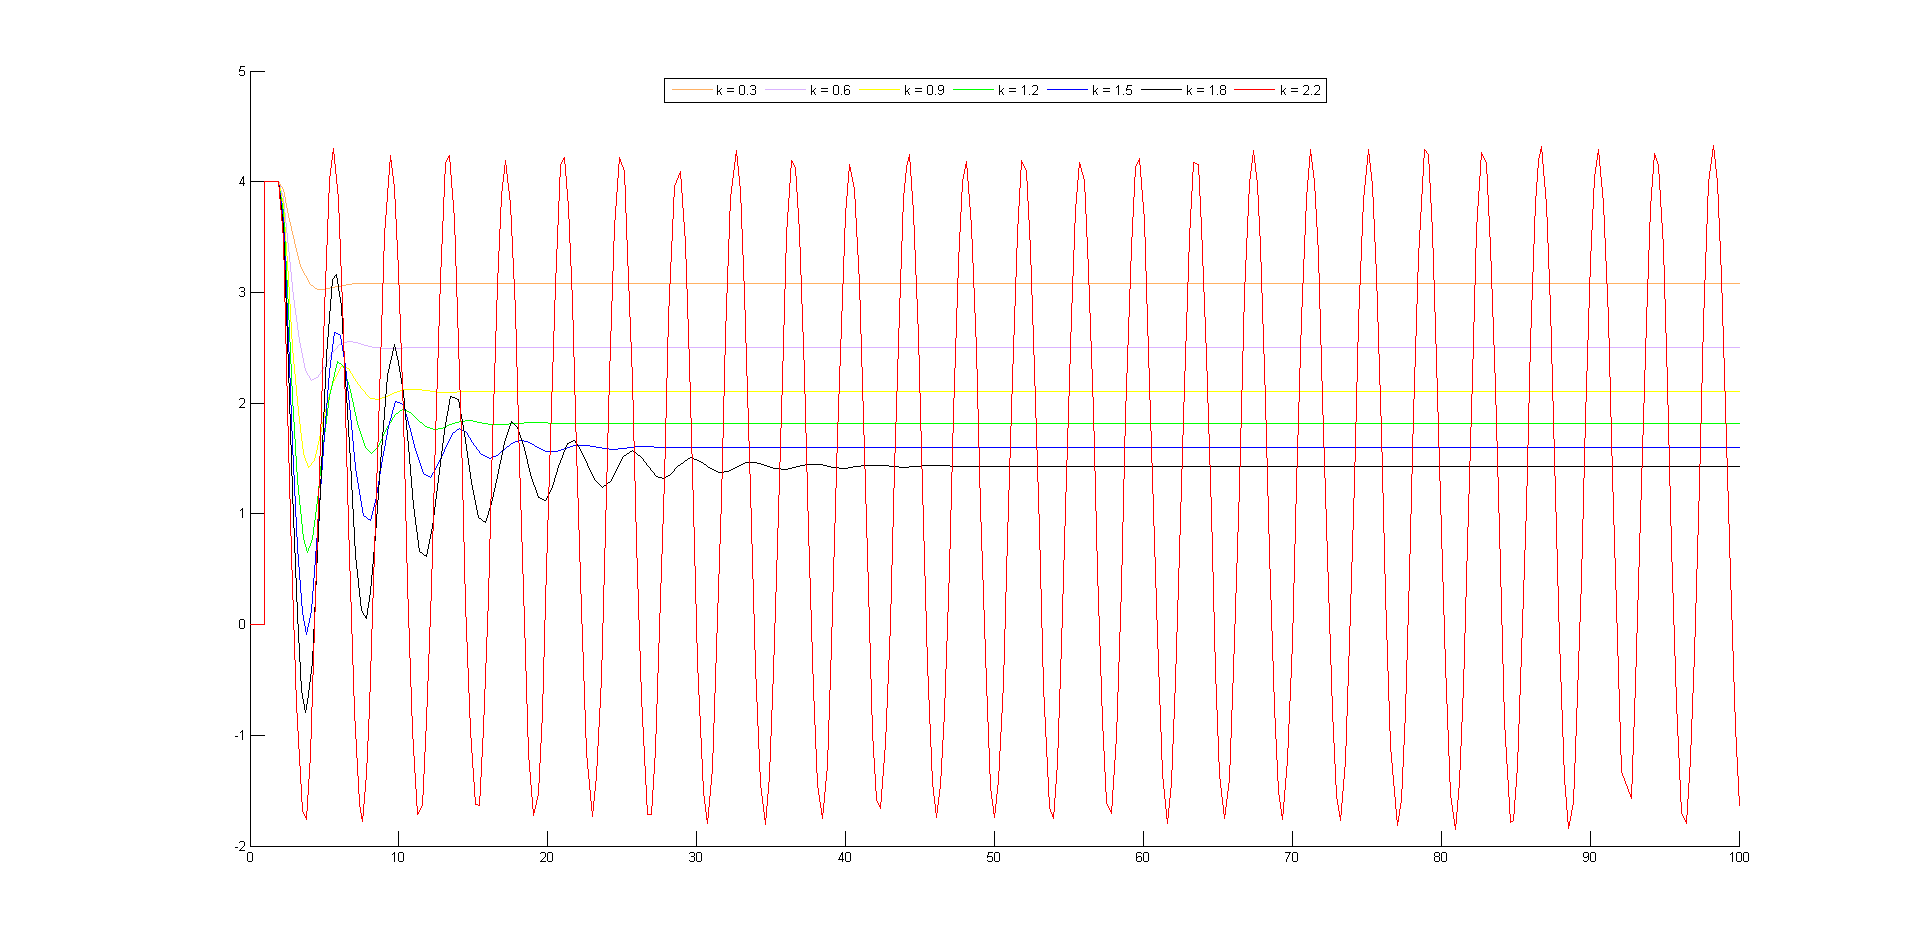
\includegraphics[width=120mm]{CW5-N3C2d1-k03-22.png}
	\caption{Wykresy przebiegu błędu regulacji przy zmianie parametru $k$}
    \label{fig:symulacjaP}
\end{figure}

Jest to sytuacja przedstawiona w poprzednim zadaniu, więc nie będziemy komentować.

\begin{figure}[!h]
    \centering
	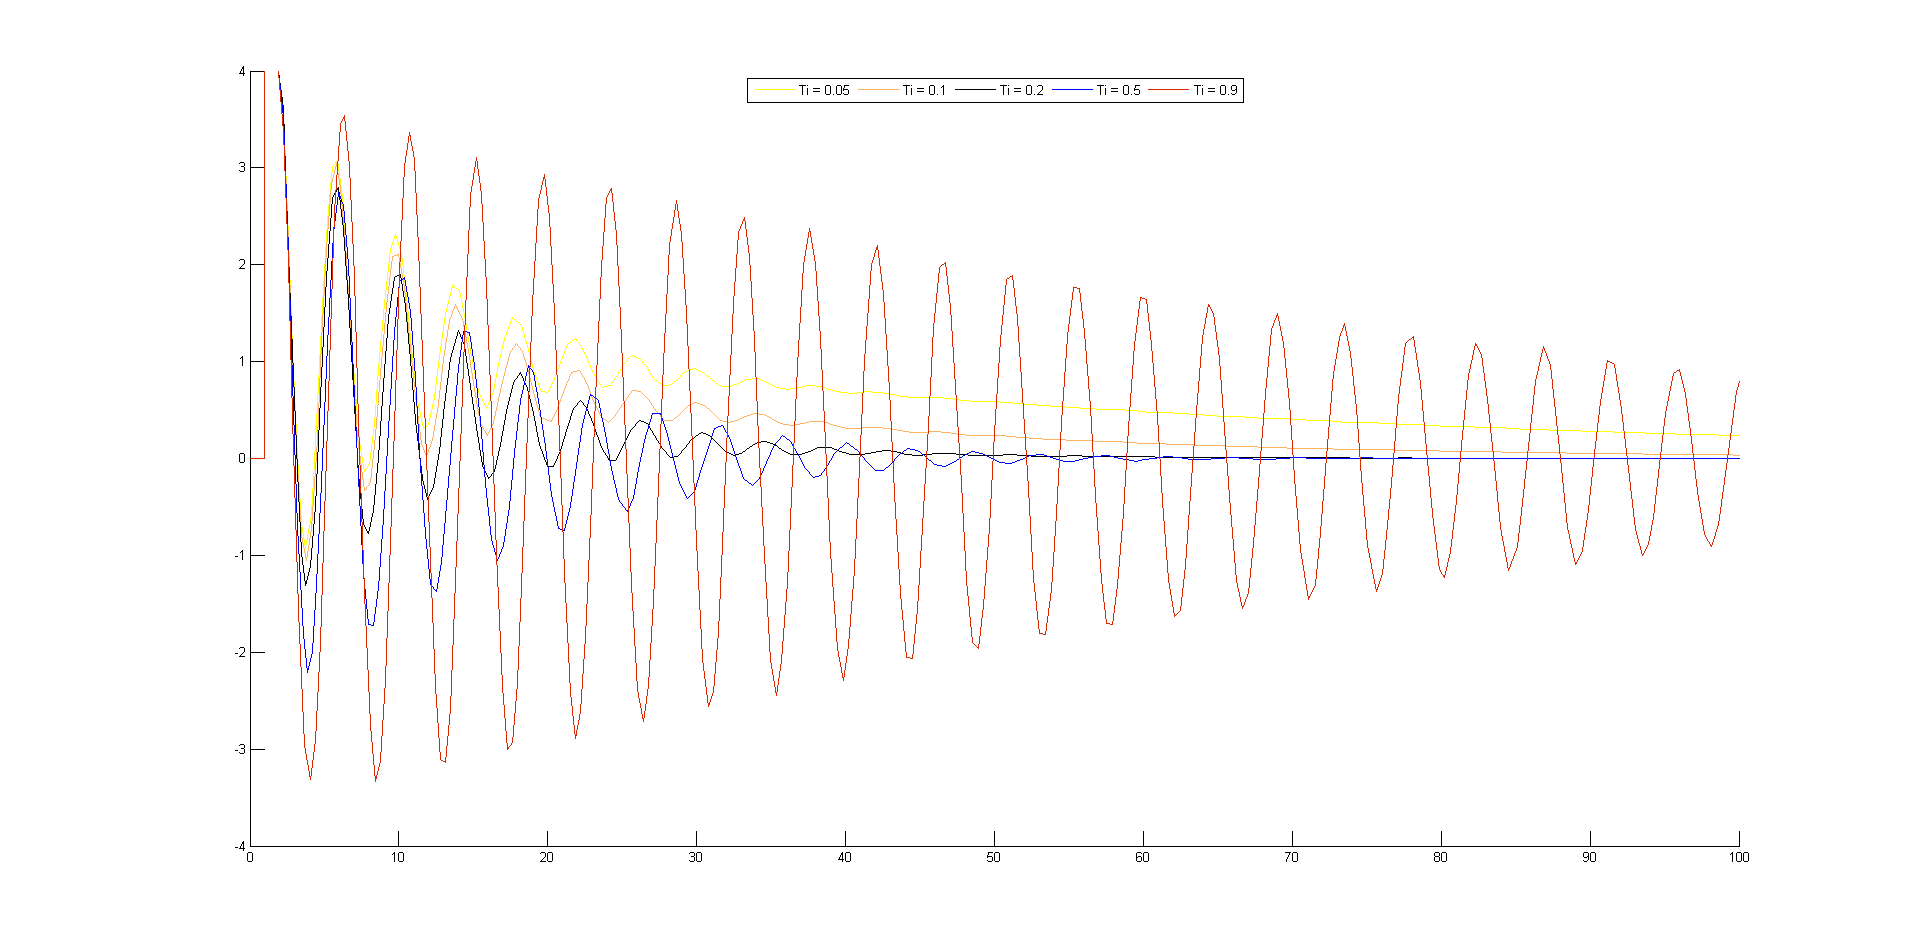
\includegraphics[width=120mm]{CW5-N3C2d1-k18-ti005-09.png}
	\caption{Wykresy przebiegu błędu regulacji przy zmianie parametru $T_i$}
    \label{fig:symulacjaP}
\end{figure}

Widać, że dzięki $T_i$ wykres zaczyna się zbliżać do 0, ale po przekroczeniu wartości $T_i \approx 0.5$ amplituda zaczyna szybko rosnąć.

\begin{figure}[!h]
    \centering
	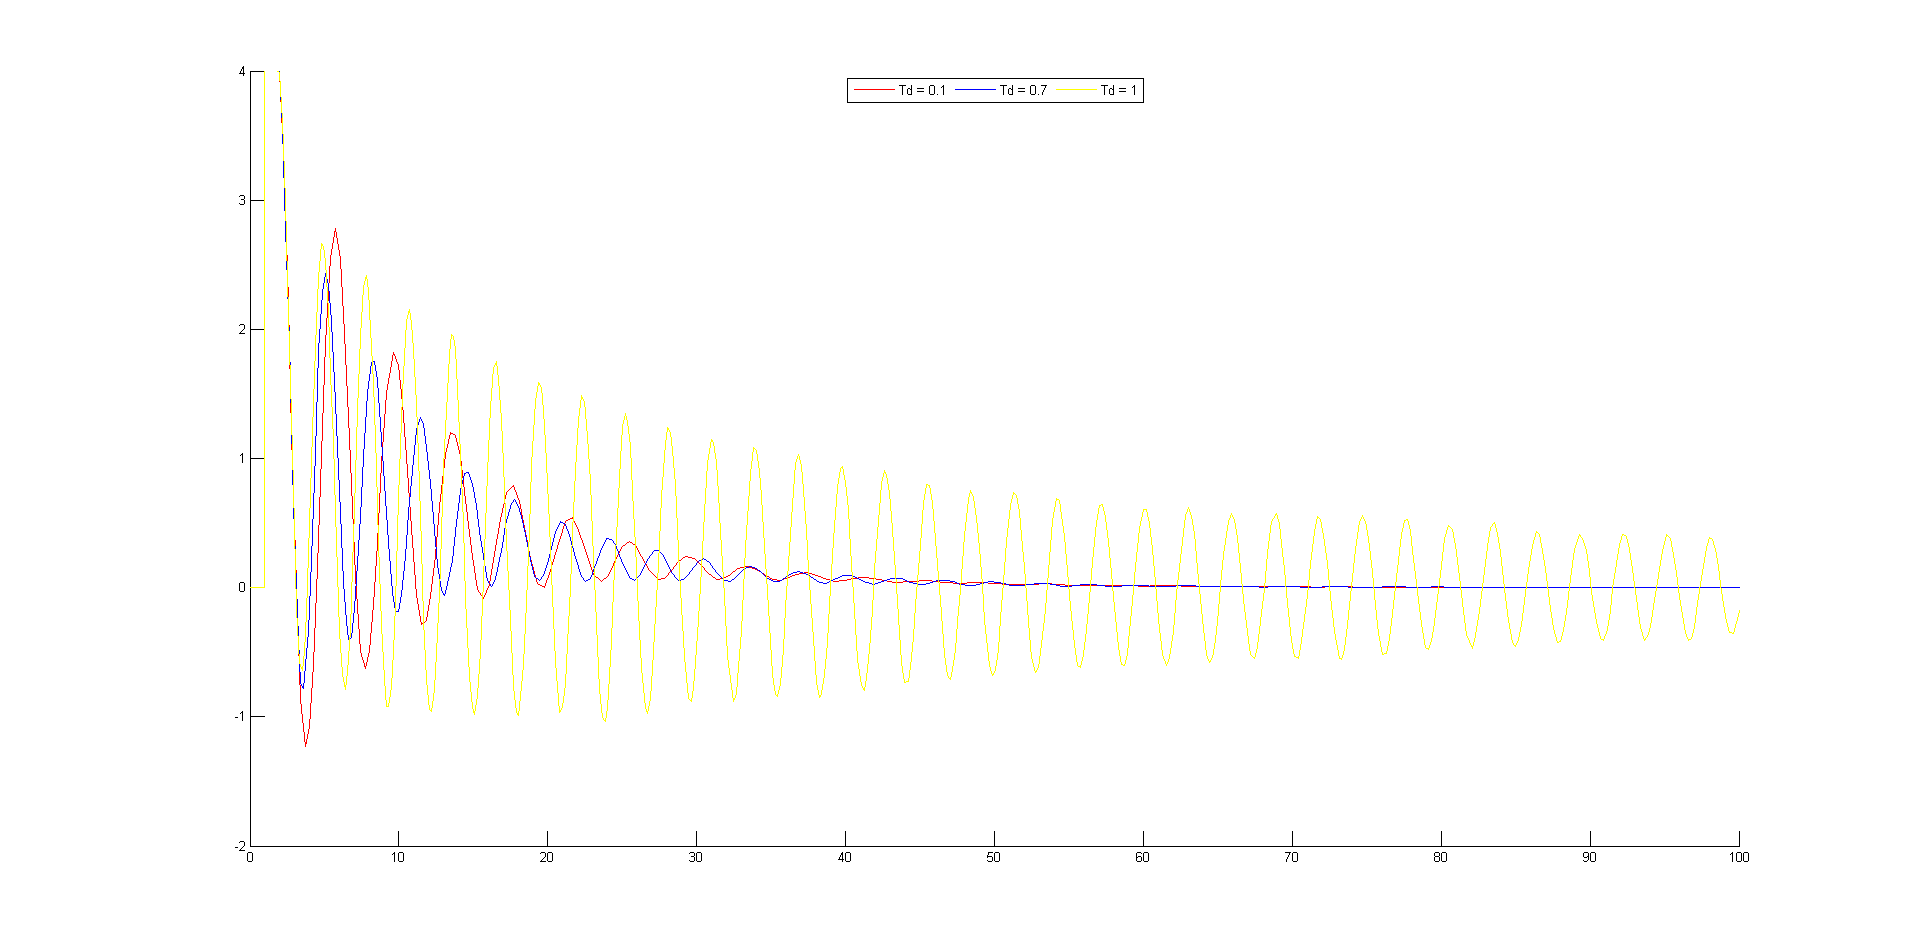
\includegraphics[width=120mm]{CW5-N3C2d1-k18-ti02-td01-1.png}
	\caption{Wykresy przebiegu błędu regulacji przy zmianie parametru $T_d$}
    \label{fig:symulacjaP}
\end{figure}
\newpage
Widać, że dzięki $T_d$ 'częstotliwość drgań' się zwiększa, ale znowu po przekroczeniu $T_d \approx 0.8$ układ się destabilizuje.

\subsubsection{Metoda Zieglera-Nicholsa}\label{sec:Mzn}
Korzystamy z metody opisanej w ćwiczeniu 2.
\begin{figure}[!h]
\begin{tabular}{ | l | c | c | c | c | c | c | }
\hline
  Typ regulatora & \multicolumn{6}{|c|}{Optymalne wartości parametrów} \\   \hline
   & \multicolumn{3}{|c|}{Próba skokowa} & \multicolumn{3}{|c|}{Granica stabilności} \\   \hline
   & $K_{p}$ & $T_{i}$ & $T_{d}$ & $K_{p}$ & $T_{i}$ & $T_{d}$\\   \hline
   P & 1/a & - & - & $0.5K_{kr}$ & - & - \\   \hline
   PI & 0.9/a & $3 T_{d}$ & - & $0.45K_{kr}$ & $T_{osc}/1.2$ & - \\   \hline
   PID & 1.2/a & $2T_{d}$ & $0.5T_d$ & $0.6K_{kr}$ & $T_{osc}/2$ & $T_{osc}/8$ \\   \hline
\hline
\end{tabular}
	\caption{Tabela Zieglera-Nicholsa}
\end{figure}
Ustaliliśmy $K_{kr}$ dla wartości:\\
$T_i = 0.5$\\
$T_d = 0.8$ \\
i wynosi 2.16

\begin{figure}[!h]
    \centering
	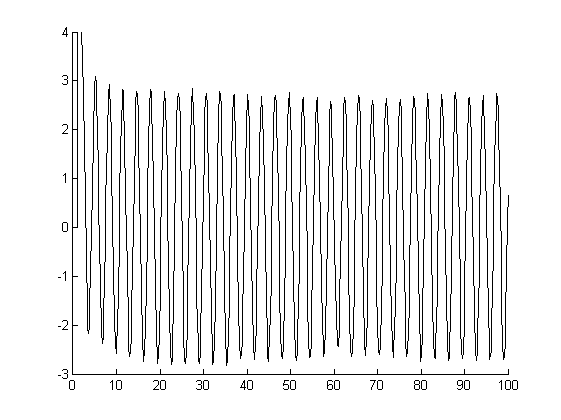
\includegraphics[width=120mm]{CW5-ZN-gs.png}
	\caption{Wykres ukłądu na granicy stabilności}
    \label{fig:symulacjaP}
\end{figure}

\begin{figure}[!h]
    \centering
	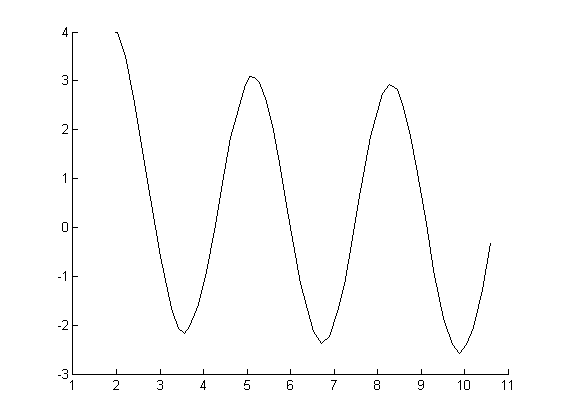
\includegraphics[width=120mm]{CW5-ZN-osc.png}
	\caption{Okres oscylacji}
    \label{fig:symulacjaP}
\end{figure}
\newpage
Rozwiązanie:\\
$K = 1.95$\\
$T_i = 1,625$\\
$T_d = 0.40625$ \\





\section{Wnioski}\label{sec:wnioski}
Ćwiczenie wykazało, że zastosowanie PID w celu regulacji transferu sieci zapewnia poprawne działanie oraz prostotę wykonania. Zaś zastosowanie regulatora P powoduje, że nie możemy efektywnie zarządzać siecią gdyż błąd regulacji nigdy się nie zeruje.
\end{document}